\documentclass[platz]{tudphygp_eng}
\usepackage{tudphymd}

\versuch{X-ray}{ROE}
\author{Jakob Kr�mer, R. Schwierz}
\bearbeitet{engl. R.Mertzig}{}
\date{17.04.2013}

\begin{document}
\maketitle

\section*{Task}

Analyze with a LiF-crystal the characteristic x-ray of copper, iron, molybdenum and wolfram. 
Identify the lines of the x-ray spectrum and calculate the corresponding energies. Discuss with your supervisor the atomic transitions corresponding to the energies measured at the respective anode materials.
 
\begin{enumerate}
 \item Use the fully equipped x-ray experiment device ``XR 4.0 expert'' for measurements.
 \item Adjust a LiF mono-crystal into the designated holder on the goniometer.
 \item Measure with the parameters shown below the counting rate of the Geiger-M�ller-counter dependent on the crystal and detector angle and plot those spectra on the computer.
 \item Analyze the spectra and identify the sharp lines.
 \item Calculate the energies of the x-rays in the found lines and determine the measurement uncertainty of the energies from the width of the lines.  
\end{enumerate}

\section*{Hints for the execution of the experiment}

\begin{itemize}
 \item Check if a x-ray tube equipped with a previously specified material is inserted in the x-ray device.

 \item  Take the 2\,mm collimator aperture from the shelf of the x-ray device (lower down) and insert it like shown in Fig.~\ref{fig:Blende} .

 Choose the LiF analyzing crystal and insert the crystal adjusting holder into the correct holes at the goniometer. The Geiger-M�ller counter, which is mounted at the end of the arm of the goniometer, will be used as the detector. 
The working voltage of the Geiger-M�ller-counter is $U = 450V$. The x-ray device can be controlled either with the control panel or connected via USB to a computer with the software \emph{measure} .\\
\begin{figure}[tbp]
\centering
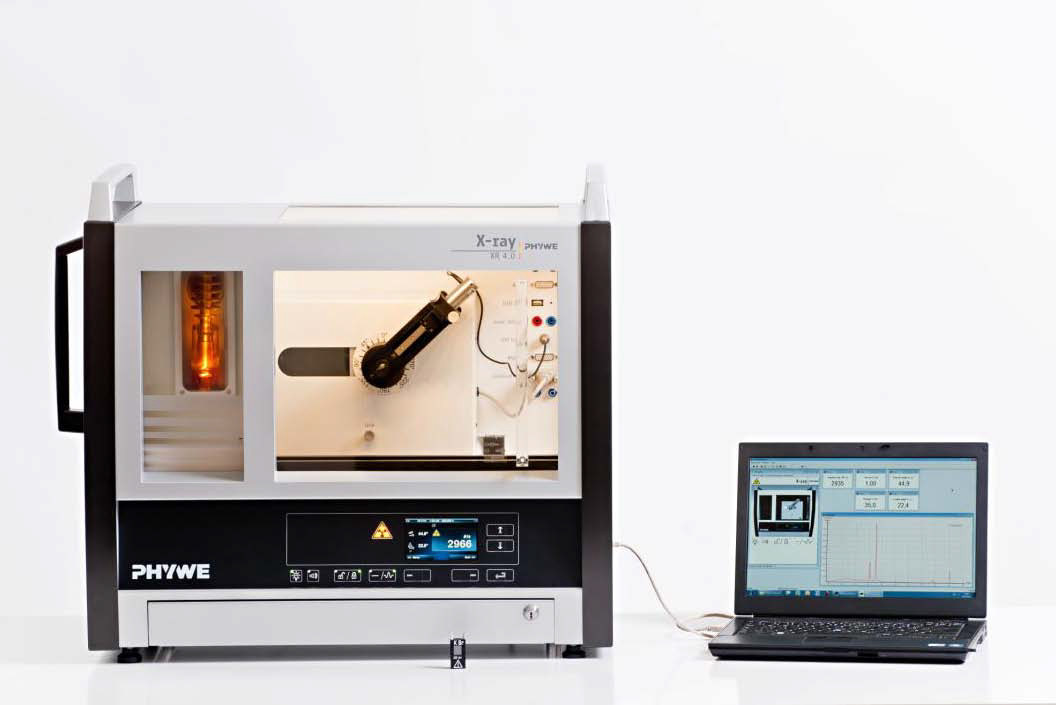
\includegraphics[width=0.8\textwidth]{images/phywe_unit.jpg}
\caption{PHYWE X-ray expert unit.}
\label{fig:messplatz}
\end{figure}
\begin{figure}[tbp]
\centering
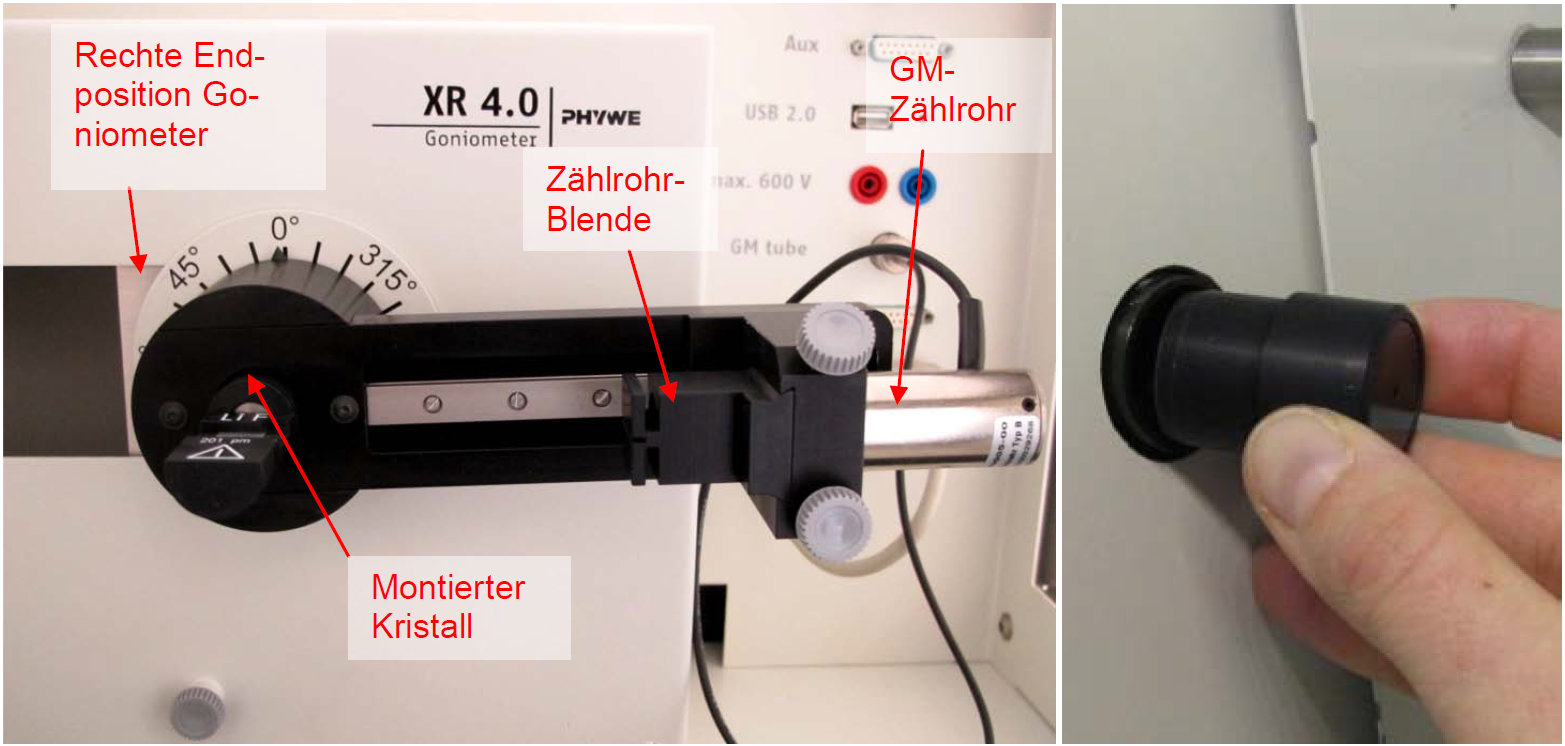
\includegraphics[width=0.8\textwidth]{images/aufbau.png}
\caption{Setup of the experimental area with the goniometer and the insertion of the collimator aperture, Source: PHYWE.}
\label{fig:Blende}
\end{figure}

 \item The x-ray device can be turned on after inserting and connecting all components.
 \item 
The goniometer has to be calibrated before starting the experiment. 
The x-ray device has to be adjusted for the usage of the LiF analysis crystal at the control panel, then the auto calibration can be started (at Goniometer - Parameter - Kristall and then Goniometer - Autokalibrierung). The auto calibration and the following measurements can be started after the glass door is closed and locked (lock symbol at the device).
\end{itemize}
The data acquisition and evaluation will be done with the program \emph{measure}. 
\begin{itemize} \item After successfully calibrating, adjust the parameter for the anode material equipped in the x-ray tube which is in use in your device at your experimental area. 

You can change the corresponding settings by clicking on the different areas of the displayed x-ray device (Abb.~\ref{fig:measure}). Check the settings of the tube, if the tube potential is adjusted to 35\,kV and emission current is adjusted to 1\,mA. The settings of the goniometer have to be adjusted according to the choice of the x-ray tube. One has to choose the angle of detection that the reflected x-rays can be measured in the glance angle.
That means that the value of the angle of detection has to be always as twice as large as the angle of the crystal (compare Fig.~\ref{fig:bragg}) . This fixed ratio is automatically kept in the mode "`1:2 Kopplung"' . 
\begin{figure}{r}[tbp]
\centering
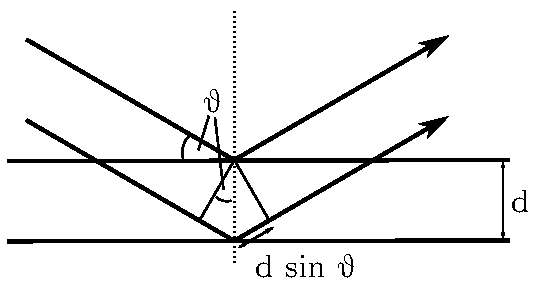
\includegraphics[width=0.4\textwidth]{images/braggdrawing.pdf}
\caption{Bragg-Reflexion im Glanzwinkel $\vartheta$ an zwei Netzebenen.}
\label{fig:bragg}
\end{figure}
\begin{figure}[tbp]
\centering
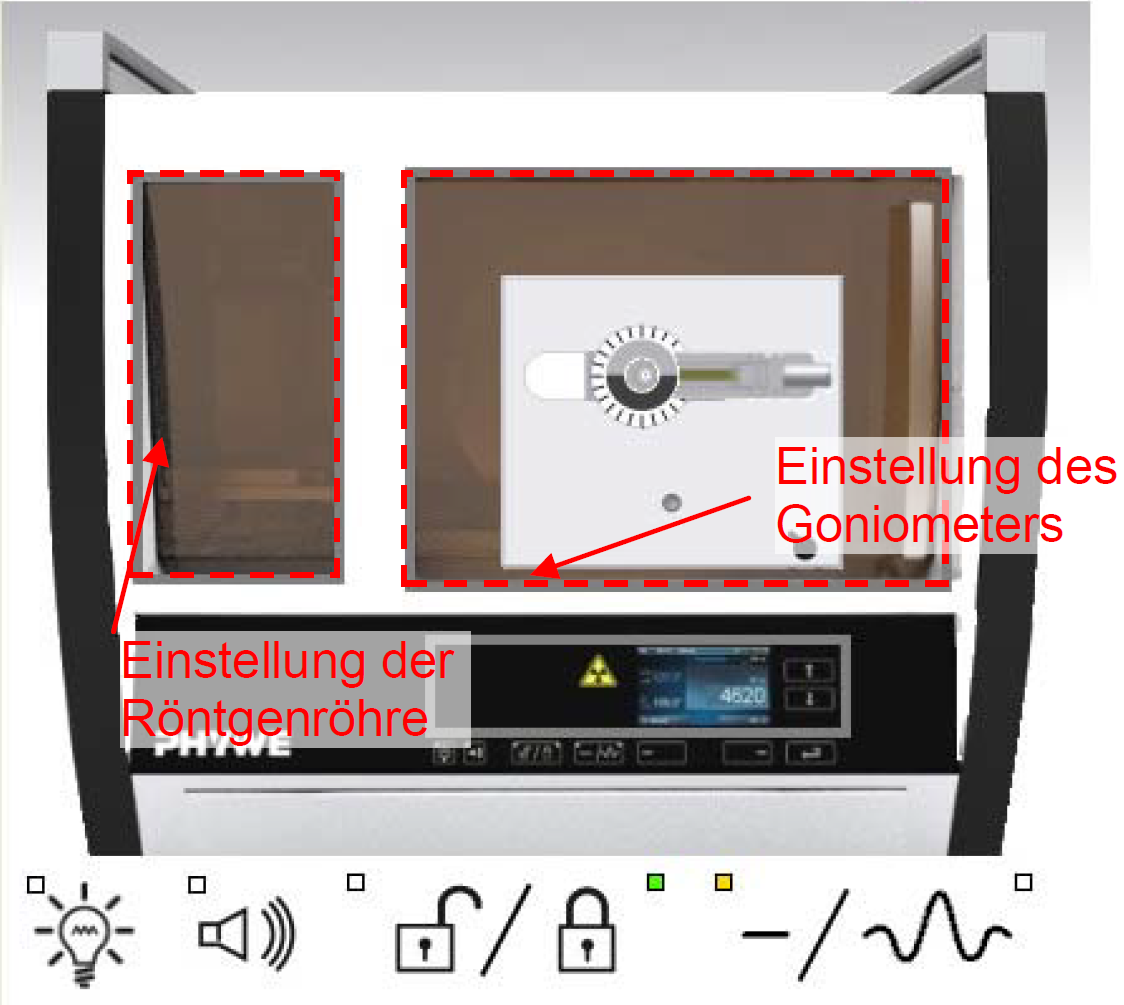
\includegraphics[width=0.5\textwidth]{images/einstellungen.png}
\caption{Tube and goniometer settings with the program \emph{measure}, Source: PHYWE.}
\label{fig:measure}
\end{figure}
\begin{figure}[tbp]
\centering
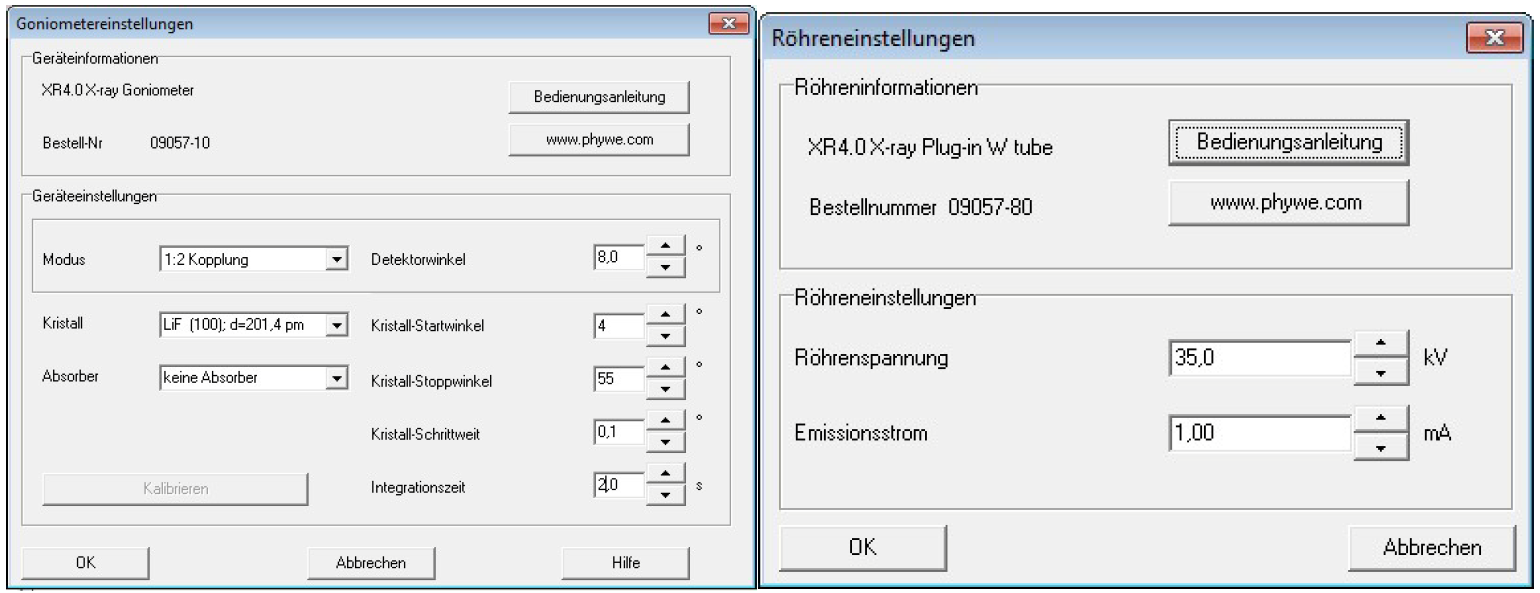
\includegraphics[width=0.9\textwidth]{images/einstellungendialog.png}
\caption{Tube and goniometer settings, Source: PHYWE.}
\label{fig:einstellungen}
\end{figure}
\begin{table}[htbp]
\begin{center}
\begin{tabular}{|l||l|r|r|r|r|}
\hline
Anode material	& Crystal	& Starting angle		& Stopping angle	& Step size	& Integration time\\
\hline\hline
Cu				& LiF		& 4�				& 55�		& 0,1�		& 2\,s\\
\hline
Fe				& LiF		& 4�				& 80�		& 0,1�		& 2\,s\\
\hline
Mb				& LiF		& 3�				& 65�		& 0,1�		& 2\,s\\
\hline
W				& LiF		& 10�				& 30�		& 0,1�		& 6\,s\\
\hline
\end{tabular}
\end{center}
\caption{Settings of the goniometer}
\label{tab:Goniometer}
\end{table}



 \item Don't adjust to any angles smaller than 3� to avoid that the Geiger-M�ller counter
is exposed to the primary beam!
 \item Click the \emph{record} button to start the experiment. Click "`alle Messungen an measure �bertragen"' after the measurement. First save your measurement and then evaluate the characteristic spectrum. For that you can use the features of \emph{measure}. Select the area of the spectrum where you want to analyze the peaks and click \emph{Peakanalyse}. Calculate the corresponding energy $E$ of the x-rays from the angles of the centers of the peaks considering their diffraction order. Calculate the corresponding measurement uncertainty $\Delta E$ of the energy from the characteristic width of the peaks.

\end{itemize}



\end{document}
